\begin{frame}{PSR estructurado por \'arbol}
    \centering
    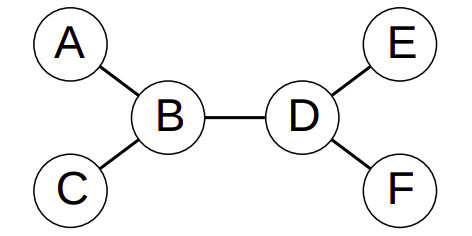
\includegraphics[width=0.4\textwidth]{34_images_CSPtree.png}\\
    \raggedright
    \emphblue{Teorema:} si el gr\'afo restricci\'on no tiene ciclos, el PSR puede ser resuelto en tiempo \textcolor{red}{$O(nd^2)$}\\
    Comparado con PSRs regulares, donde el costo de tiempo para el peor caso es \textcolor{red}{$O(d^n)$}\\
    
    Esta propiedad tambi\'en aplica a un razonamiento l\'ogico y probabil\'istico:\\
    
    un ejemplo importante de la relaci\'on entre las restricciones sint\'acticas y la complejidad de razonamiento
\end{frame}
